\documentclass[12pt]{article}

\usepackage{sbc-template}
\usepackage{graphicx,url}
\usepackage{microtype}
\usepackage[utf8]{inputenc}
\usepackage[brazil]{babel}
\usepackage{comment}
\usepackage{lipsum}
\usepackage{csquotes}
\usepackage{url}
\usepackage{placeins}
\usepackage[
    style=authoryear,
    citestyle=authoryear,
    backend=biber
]{biblatex}

\addbibresource{references.bib}

\DeclareFieldFormat{labelyear}{#1}
\renewcommand*{\nameyeardelim}{\addspace}
\renewbibmacro*{cite}{%
  \printtext[brackets]{%
    \printnames{labelname}%
    \setunit{\nameyeardelim}%
    \printfield{labelyear}%
  }}

\urlstyle{same} 

\sloppy

\title{Análise comparativa de métricas de avaliação\\
em modelos de aprendizado de máquina na detecção de\\
ataques de spoofing de GPS
}

\author{Ana Carla Rodrigues\inst{1}, Jessica Fileto\inst{1}}

\address{
  Centro de Matemática, Computação e Cognição\\
  Universidade Federal do ABC (UFABC)\\
  Av. dos Estados, 5001 -- 09210-580 -- Santo André -- SP -- Brasil
  \email{\{carla.rodrigues,jessica.fileto\}@ufabc.edu.br}
}

\begin{document}

\maketitle
     
\begin{resumo} 
O Veículo Aéreo Não Tripulado (VANT), comumente conhecido como drone, é uma
plataforma que está revolucionando indústrias ao redor do mundo, oferecendo 
soluções de alta flexibilidade e riscos reduzidos. O Global Positioning System 
(GPS) fornece ao VANT navegação precisa, rastreamento e vôo autônomo. Os VANTs 
podem sofrer ataques de spoofing nas coordenadas de GPS, comprometendo a 
segurança da informação e demonstrando que a precisão na análise dos dados são 
cruciais na tomada de decisões. A inteligência artificial pode ser uma aliada 
na detecção destes ataques através de técnicas sofisticadas, reduzindo a 
quantidade de falsos alarmes e fornecendo informações confiáveis por meio do 
aprendizado de máquina que exerce papel fundamental na classificação destes 
ataques. A proposta deste projeto é realizar uma análise comparativa das 
métricas de avaliação dos seguintes modelos de aprendizado de máquina:
Random Forest, XGBoost, SVM, K-NN,
Gaussian Naive Bayes e Extremely Randomized Trees,
visando identificar aquele que melhor equilibre a detecção correta
de spoofing e viabilidade de implementação do modelo.
\end{resumo}

\section{Introdução}

Os veículos aéreos não tripulados (VANTS), também conhecidos como drones,
são um tipo de tecnologia fundamental tanto em áreas civis quanto militares.
Seu uso reduz a exposição humana a tarefas repetitivas, de longa duração
e em alguns casos, de alto risco \cite{dialogos}.
Desempenham papel importante nas seguintes áreas: gerenciamento de desastres,
vigilância aérea, fotografia aérea de rastreamento, pesquisa e resgate,
monitoramento de gado, dentre outros. \cite{titounaLightweightSecurityTechnique2021} 

Por serem operados de maneira autônoma e remota suas coordenadas são essenciais
para o sucesso de suas missões, para isso são usados sinais
de Sistema Global de Navegação por Satélite (GNSS),
sendo o mais conhecido o \textit{Global Positioning System} (GPS),
esses sinais podem ser criptografados ou não \cite {lester}.
Sendo os não criptografados mais suscetíveis a ataques conhecidos como
\textit{Spoofing} de GPS \cite{srinivasansGPSSpoofingDetection2023}.

O ataque de \textit{spoofing} de GPS
é caracterizado por um atacante que faz uso de antenas terrestres
emitindo sinais falsos. \cite{Spoofing}
Estes ataques são classificados em: simples,
intermediários e sofisticados \cite{Aissou2021}.

Para garantir um vôo seguro do VANT é essencial ter medidas
para detecção dos ataques de \textit{Spoofing de GPS}.
A identificação precisa desses ataques é extremamente importante,
pois técnicas sofisticadas de \textit{spoofing}
podem causar disrupção no funcionamento do VANT,
portanto são necessários métodos robustos e adaptativos
\cite{isleyenGPSSpoofingDetection2024}.
Nesse contexto algoritmos de aprendizado
de máquina tem se mostrado promissores,
pois são capazes de analisar grandes volumetrias de dados,
identificando padrões e anomalias.
Tais abordagens oferecem uma resposta robusta e adaptativa
a essas ameaças contribuindo para as operações dos VANTs
\cite{isleyenGPSSpoofingDetection2024}.

Neste trabalho será feita a reimplementação dos algoritmos
\textit{RandomForest} e \textit{XGBoost} e seus respectivos 
experimentos do artigo \cite{Aissou2021}, com o objetivo de comparar
esses algoritmos com outros que não são baseados em árvore,
sendo eles: \textit{Support Vector Machines} (SVM), \textit{K-NN},
\textit{Gaussian Naive Bayes} e \textit{Extremely Randomized Trees}.

\section{Trabalhos relacionados}

Diversos estudos recentes tem utilizado aprendizado de máquina
para detecção de ataques de \textit{spoofing} de GPS.
Podemos mencionar algumas abordagens utilizadas:

\begin{itemize}
    \item \textbf{Redes neurais profundas (DNN):}
     Extração de padrões complexos em séries temporais dos sinais GNSS.
     \cite{isleyenGPSSpoofingDetection2024}

    \item \textbf{Máquinas de vetores de suporte (SVM):}

     Abordagem teve como objetivo a identificação
     de discrepâncias entre as posições determinadas pelos sinais de GPS
     e aquelas medidas pelo sistema de navegação inercial (INS).
     Especificamente, o modelo SVM foi treinado através dos erros obtidos
     das diferenças posicionais,
     permitindo que o sistema detecte inconsistências que poderiam
     indicar um ataque de \textit{spoofing} de GPS.
     \cite{panice2017}
    
    \item \textbf{Redes neurais convolucionais (CNN):} Em comparação
    aos modelos tradicionais de aprendizagem de máquina,
    os de aprendizagem profunda obtiveram alta acurácia na detecção dos
    ataques de \textit{spoofing}.
    A grande vantagem desses modelos baseados em aprendizagem profunda,
    é pelo fato de aprenderem automaticamente a extraírem as \textit{features}
    sem precisarem de intervenção humana. Além de se adaptarem melhor
    a \textit{datasets} mais complexos. \cite{cnn2023}

    
    \item \textbf{Aprendizagem supervisionada (Baseado em Árvores):}
    \textcite{Aissou2021} utilizou os seguintes modelos baseados
     em árvores: Random Forest, Gradient Boost, XGBoost e LightGBM
     para fazer um comparativo de qual seria melhor na detecção dos ataques
     de \textit{spoofing} de GPS.
     Sendo que o XGBoost obteve a melhor acurácia (95,52\%).

    \item \textbf{IA Generativa:}  Abordagem que em comparação com outros
    modelos de aprendizagem de máquina, se destacou pela eficácia
    na deteção dos ataques de \textit{spoofing} e \textit{jamming}.
    \cite{elalamiDroneDefGANtGenerativeAIBased2024}
    
\end{itemize}

\section{Delimitação e Escopo}

O artigo \cite{Aissou2021} não cita o \textit{dataset}
usado para o treinamento dos modelos, 
então para as análises decorrentes deste artigo
será utilizado o \textit{Mendeley Data} 
\cite{aissou2022dataset}, que foi disponibilizado pelos autores do artigo. 
Esse \textit{dataset} é uma versão simplificada,
pois é representada em duas dimensões. Esses dados foram gerados de sinais
GPS autênticos e contém aproximadamente 500,000 dados.

Nas próximas seções se estabelecerá a execução do trabalho.
Na seção 4, faremos nossa proposta de mudança
ao trabalho de \cite{Aissou2021}, discutindo a 
metodologia e modelos de aprendizado de máquina a
serem implementados. Logo, os resultados e 
discussões serão apresentados na seção 5.
Finalmente, nossas conclusões sobre o trabalho serão expostos na seção 6.

\section{Metodologia}
A metodologia adotada e os passos seguidos
foram inspirados no artigo de \cite{Aissou2021}, 
que implementou os algoritmos baseados em árvore: 
\textit{Random Forest}, \textit{Gradient Boost}, \textit{XGBoost}, e 
\textit{LightGBM} com o objetivo de explorar os dados obtidos.

Será realizada a reimplementação dos algoritmos
(i) \textit{Random Forest} e (ii) \textit{XGBoost},
ambos obtiveram o pior e melhor desempenho,
respectivamente, ponderando as métricas de tempo de execução
e uso de memória, no comparativo dos modelos baseados em árvore.
Ambos algoritmos serão comparados com outros
modelos que não são baseados em árvore,
sendo eles: (iii) SVM, (iv) \textit{K-NN} e
(v) \textit{Gaussian Naive Bayes}.

Será incluído o modelo baseado em árvore conhecido como
(vi) \textit{Extremely randomized trees} que é um modelo melhorado
do \textit{Random Forest}, que se difere pelo fato
que no \textit{Extremely randomized trees} não existe a fase
de \textit{bagging} e no momento da separação dos nós,
esta escolha é feita aleatoriamente \cite{geurtsExtremelyRandomizedTrees2006}.

Será feita a análise comparativa entre os algoritmos baseados em árvore
e os demais algoritmos, com o objetivo de identificar
aquele que melhor equilibre a detecção correta
de \textit{spoofing} e viabilidade de implementação do modelo.
Também ocorrerá a análise entre os modelos baseados em árvore
para averiguar se o \textit{Extremely Randomized Trees}
obtém um desempenho melhor que o \textit{Random Forest}.
O algoritmo \textit{XGBoost}
será mantido, pois obteve o melhor desempenho
no artigo de \cite{Aissou2021}.
Portanto ele será usado como base
para comparação com os demais algoritmos.

Para a avaliação do desempenho dos modelos
será utilizada a biblioteca \textit{PyCM} do Python,
que é uma biblioteca de matriz de confusão
multiclasse, que implementa diversas métricas de classificação.
\cite{Haghighi2018}

Serão analisadas a acurácia,
precisão e a quantidade de falsos negativos.
Além disso, será feita a análise do tempo de treinamento,
predição e uso de memória de cada modelo,
com o objetivo de identificar o mais viável
para implementação em VANTs.

\subsection{Divisão dos dados}
A base será dividida em porções
diferentes para testes e o treinamento do modelo,
sendo 70\% para treino e 30\% para testes
conforme realizado no artigo. \cite{Aissou2021}

\subsection{Matthews Correlation Coefficient (MCC)}
O \textit{Matthews Correlation Coefficient} (MCC) é uma métrica
de avaliação de modelos de classificação binária,
que posteriormente foi extrapolada para classificação multiclasse. \cite{MCC}

Neste trabalho será utilizado o MCC,
juntamente com a acurácia para avaliar a eficácia
dos modelos de aprendizado de máquina
na detecção de ataques de \textit{spoofing} de GPS.

\subsection{Pré-Processamento dos dados}

Será aplicada a técnica de pré processamento
\textit{Principal Component Analysis} (PCA) para melhorar
a precisão dos resultados finais. Ela consiste em reduzir a
dimensão do dataset para deixar apenas as informações mais relevantes,
removendo assim as redundâncias \cite {pearson1901}. 
Assim como serão utilizadas
outras duas técnicas adicionais conhecidas como \textit{Standard Scaler} para
melhorar o desempenho do processamento \cite {pearson1901} e o
\textit{Random Under Sampler} para reduzir o desbalanceamento das classes
que dificultam o treinamento e a análise dos dados \cite {japkowicz2000}.

Essas técnicas são
diferentes da usada no artigo de \cite{Aissou2021}
que se chama \textit{Spearman Correlation Coefficient}.

\subsection{Análise do desempenho}
Para análisar a eficácia do algoritmo através dos dados disponíveis é 
necessário avaliar os comportamentos dos modelos e para isso 
serão utilizadas as seguintes métricas:
(\romannumeral 1) probabilidade de detecção,
(\romannumeral 2) acurácia,
(\romannumeral 3) probabilidade de detecção falsa,
(\romannumeral 4) probabilidade de alarme falso,
(\romannumeral 5) taxa de erro,
(\romannumeral 6) coeficiente MCC,
(\romannumeral 7) F1 score,
(\romannumeral 8) especificidade.

\section{Resultados e discussões}

\begin{figure}[ht]
  \centering
  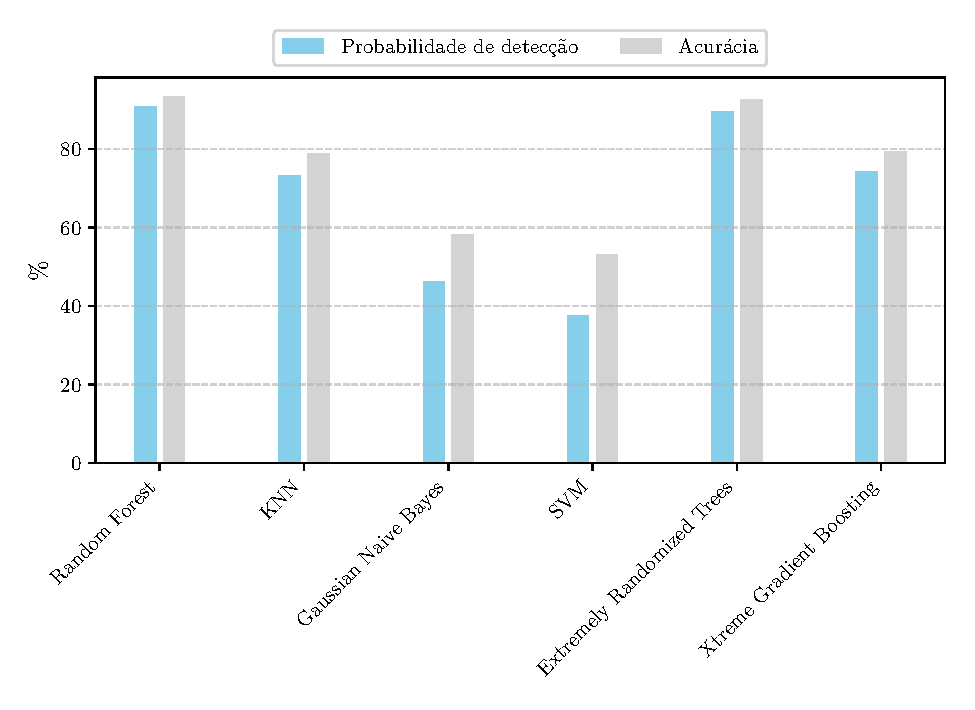
\includegraphics[width=1\linewidth]{../plot_accuracy_and_tpr.pdf}
  \caption{Gráfico de probabilidade de detecção e acurácia.}
\end{figure}

\begin{figure}[ht]
    \centering
    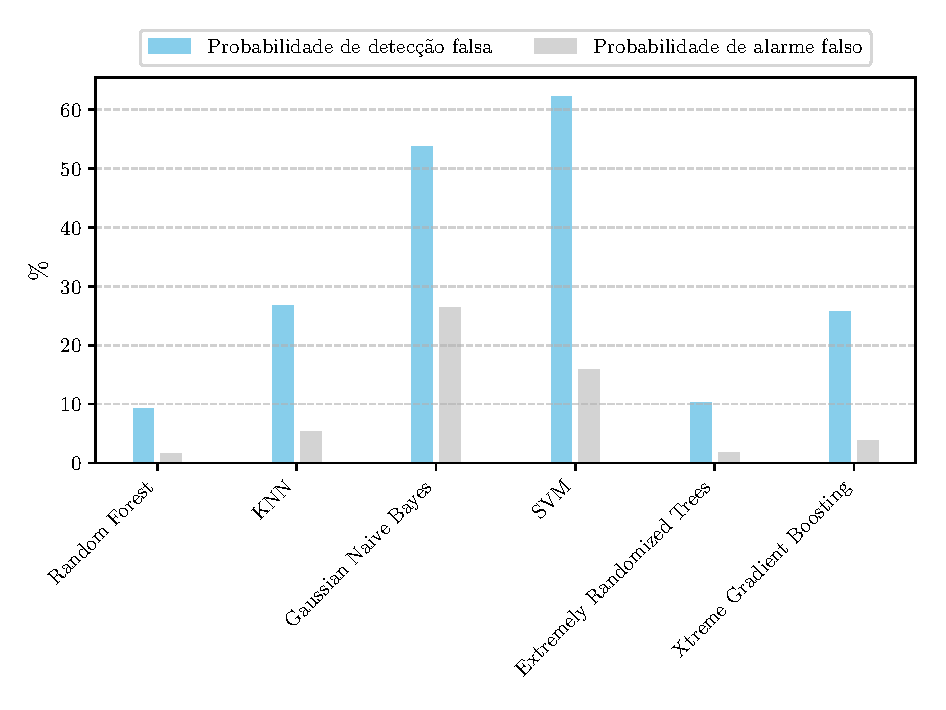
\includegraphics[width=1\linewidth]{../plot_pmd_and_pfa.pdf}
    \caption{Gráfico de probabilidade de detecção falsa e probabilidade de alarme falso.}
\end{figure}

\begin{table}
  \caption{Métricas de performance dos modelos}
  \resizebox{\textwidth}{!}{%
    \begin{tabular}{|l|l|l|l|l|}
      \hline
      Algoritmo & Tempo de treinamento & Uso de memória (treinamento) & Tempo de predição & Uso de memória (predição) \\
      \hline
      Gaussian Naive Bayes & 209.44 ms & 8.92 MiB & 48.67 ms & 33.95 MiB \\
      KNN & 335.34 ms & 4.18 MiB & 9129.37 ms & 25.39 MiB \\
      SVM & 772.69 ms & 1.45 MiB & 15.19 ms & 9.41 MiB \\
      Extremely Randomized Trees & 6180.53 ms & 10.12 MiB & 2237.85 ms & 18.13 MiB \\
      Random Forest & 43128.56 ms & 11.84 MiB & 1475.68 ms & 18.13 MiB \\
      Xtreme Gradient Boosting & 229203.56 ms & 18.13 MiB & 793.14 ms & 23.96 MiB \\
      \hline
    \end{tabular}
  }
\end{table}

\begin{table}
  \caption{Métricas de desempenho}
  \resizebox{\textwidth}{!}{%
    \begin{tabular}{|l|l|l|l|l|l|l|l|}
      \hline
      Métrica & Random Forest & Extremely Randomized Trees & XGBoost  & KNN & Gaussian Naive Bayes & SVM \\
      \hline
      Probabilidade de detecção & 90.76\% & 89.71\% & 74.31\% & 73.32\% & 46.21\% & 37.68\% \\
      Acurácia & 93.51\% & 92.65\% & 79.29\% & 78.96\% & 58.31\% & 53.25\% \\
      Probabilidade de detecção falsa & 9.24\% & 10.29\% & 25.69\% & 26.68\% & 53.79\% & 62.32\% \\
      Probabilidade de alarme falso & 1.63\% & 1.74\% & 3.79\% & 5.37\% & 26.45\% & 15.95\% \\
      Taxa de Erro & 6.49\% & 7.35\% & 20.71\% & 21.04\% & 41.69\% & 46.75\% \\
      Coeficiente MCC & 0.81 & 0.79 & 0.57 & 0.55 & 0.16 & 0.18 \\
      F1-Score & 0.91 & 0.90 & 0.77 & 0.76 & 0.53 & 0.45 \\
      Especificidade & 0.98 & 0.98 & 0.96 & 0.95 & 0.74 & 0.84\\
      \hline
    \end{tabular}
    }
\end{table}


\FloatBarrier

Com base nos dados da Tabela 1 podemos avaliar o desempenho dos algoritmos utilizados 
para classificar ataques de \textit{spoofing} aos VANTS.
\subsection{Probabilidade de detecção}
\subsection{Acurácia}
\subsection{Probabilidade de detecção falsa}
\subsection{Probabilidade de alarme falso}
\subsection{Taxa de erro}
\subsection{Coeficiente MCC}
\subsection{F1 score}
\subsection{Especificidade}

\section{Conclusão}

\printbibliography

\end{document}
